\begin{frame}{Cấu hình tài nguyên Kubernetes trong GitOps Repository}
\begin{figure}[H]
\centering
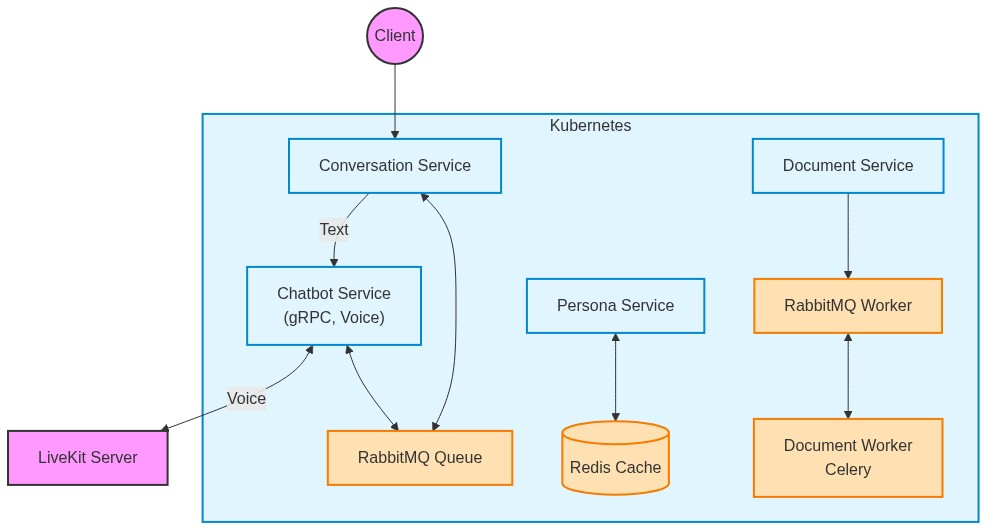
\includegraphics[height=0.55\textheight,width=0.9\textwidth,keepaspectratio]{pictures/Kubernetes.png}
\caption{Cấu hình Kubernetes trong kho lưu trữ GitOps của dự án}
\end{figure}

\note{
Đây là cấu trúc thư mục chứa các file cấu hình Kubernetes (YAML) trong kho lưu trữ GitOps của dự án.
Các dịch vụ nội bộ như RabbitMQ, Redis được chạy trực tiếp trong cụm để giảm độ trễ và được cấu hình dưới dạng ClusterIP để tăng tính bảo mật, ngăn chặn các truy cập trực tiếp từ internet. Các dịch vụ chạy bất đồng bộ như Voice Agent hay Document Worker cũng không công khai service ra bên ngoài.
}
\end{frame}
